\documentclass[12pt,a4paper]{article}
\usepackage{amsmath}
\usepackage{amssymb}
\usepackage{graphicx}

\topmargin  -18mm    
\textheight 254mm   
\textwidth 169mm    
\oddsidemargin -4mm
\begin{document}
\begin{center}
{\Large \textbf{Truncated Jacobi operators}}\\
{\footnotesize \today}
\end{center}

\noindent On the upper branch of the teardrop curve,
\begin{equation*}
\gamma = \left\lbrace (x,y): y^2 = \phi(x) := \frac{1}{4}(1 - x)^2(1+x),\: y\geq 0, \: -1 \leq x \leq 1\right\rbrace,
\end{equation*}
with the inner product,
\begin{equation*}
\langle f,g \rangle = \int_{-1}^{1} fg\left(x,\sqrt{\phi(x)}\right) w_{\alpha,\beta}(x)\mathrm{d}x, \qquad w_{\alpha,\beta}(x) = (1-x)^{\alpha}(1+x)^{\beta},
\end{equation*}
we do not have an explicit OP basis but we can construct it with the Gram-Schmidt procedure. The orthonormalized OP basis satisfies 
\begin{equation*}
x Q_n = B^{\intercal}_{n-1,1}Q_{n-1} + A_{n,1}Q_n + B_{n,1}Q_{n+1},
\end{equation*}
\begin{equation*}
y Q_n = B^{\intercal}_{n-1,2}Q_{n-1} + A_{n,2}Q_n + B_{n,2}Q_{n+1}.
\end{equation*}
The Jacobi operators are asymptotically, as $n \to \infty$, block-Toeplitz with $3\times3$ blocks.
Let $A^x = \lim_{n \to \infty}A_{n,1}$ and let $A^y, B^x, B^y$ be similarly defined. For $\alpha = \beta = -1/2$, we find that
\begin{equation}
A^x = 
\frac{1}{8}\left(
\renewcommand{\arraystretch}{1.0}
\begin{array}{r r r}
-2 & -4 & -1\\
-4 & -2 & 4\\
-1 & 4  & -2
\end{array}
\right), \qquad
B^x = \frac{1}{8} \left(
\renewcommand{\arraystretch}{1.0}
\begin{array}{r r r}
0 & 0 & 0\\
1 & 0 & 0\\
4 & -1  & 0
\end{array}
\right),
\label{eq:xlimmats}
\end{equation}
and
\begin{equation}
A^y = v\left(
\renewcommand{\arraystretch}{1.0}
\begin{array}{r r r}
12 & -1 & 6 \\
-1 & 12 & 1 \\
6 & 1 & 12
\end{array}
\right)
, \qquad
B^y = 
v\left(
\renewcommand{\arraystretch}{1.0}
\begin{array}{r r r}
1 & 0& 0\\
-6& 1 &0\\
1 &6& 1
\end{array}
\right),
\qquad
v = \frac{\sqrt{2}}{64}.
\label{eq:ylimmats}
\end{equation}
The symbols associated with the limiting $x$ and $y$ Jacobi operators are, respectively,
\begin{equation*}
X(z) = \frac{\left(B^x\right)^{\intercal}}{z} + A^x + B^x z, \qquad
Y(z) = \frac{\left(B^y\right)^{\intercal}}{z} + A^y + B^y z, 
\end{equation*}
where $z$ is on the complex unit circle. The symbols commute, satisfy the algebraic equation defining $\gamma$ and the image of their joint spectrum is the support of the OPs (also $\gamma$), i.e., 
\begin{equation*}
X(z)Y(z) = Y(z)X(z), \qquad Y(z)^2 = \phi\left[X(z) \right] = \frac{1}{4}\left[\,\mathrm{I} - X(z)\,\right]^2\left[\,\mathrm{I} + X(z)\,\right],
\end{equation*}
and
\begin{equation}
\left\lbrace (\lambda_{x,i}, \lambda_{y,i}) \: : \:  X(z)q_i = \lambda_{x,i} q_i, \: Y(z)q_i = \lambda_{y,i} q_i, \: \lambda_{y,i} = \sqrt{\phi(\lambda_{x,i})}, \: i = 1, 2, 3,\: \vert z \vert = 1 \right\rbrace = \gamma
\label{eq:jointspect}
\end{equation}
see Figure~\ref{fig:symbolspectrum}.
\begin{figure}
	\centering
	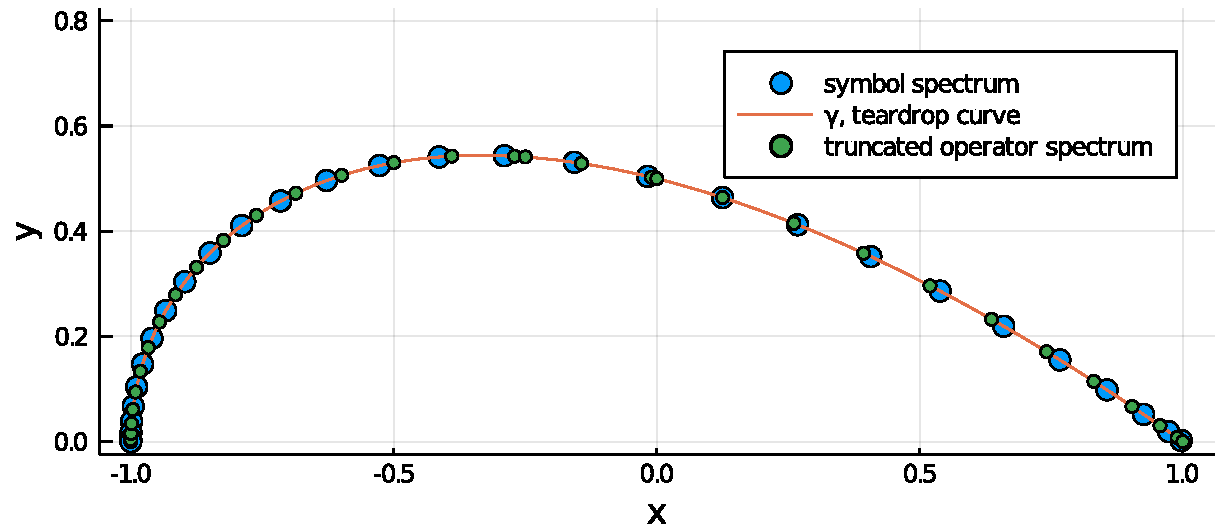
\includegraphics[width = 0.9\textwidth]{symbol_spectrum2.pdf}
	\caption{In blue, the joint spectrum of $X(z)$ and $Y(z)$, i.e., a plot of $(\lambda_{x,i}, \lambda_{y,i})$ defined in (\ref{eq:jointspect}), sampled at $20$ equally spaced points on the complex unit circle. In green, the joint spectrum of $33 \times 33$ versions of the truncated operators $\widetilde{X}$ and $\widetilde{Y}$ defined in (\ref{eq:xtruncation})--(\ref{eq:opspectrum}).   }   
	\label{fig:symbolspectrum}
\end{figure}

It is possible to construct truncated versions of the limiting $3\times 3$-block-Toeplitz Jacobi operators in such a way that they commute and satisfy the algebraic equation defining the teardrop curve. The truncated operators take the form
\begin{equation}
\widetilde{X} := \left(
\begin{array}{c c c c c c c c }
A_0^x  & B_0^x   &        &        & & & &   \\
\left(B_0^x \right)^{\intercal} & A_1^x  & B_1^x &       & &  & &      \\
                                &\left(B_1^x \right)^{\intercal} & A^x  &  B^x       &  &    & &     \\
                                            & & \left(B^x \right)^{\intercal}  &  \ddots        & \ddots  &  & &       \\
                                                        & &    &   \ddots      & \ddots  &B^x   & &       \\
             & &   &          & \left(B^x \right)^{\intercal}  &      A^x    & \left(b_1^x \right)^{\intercal} &  \\
                                &                        & &          &  & b_1^x   & a_1^x & \left(b_0^x \right)^{\intercal}  \\
                                &     & & & &  &  b_0^x & a_0^x
\end{array}
\right), \label{eq:xtruncation}
\end{equation}
where $A_0^x$, $a_0^x$ are $1\times 1$ matrices; $B_0^x$, $b_0^x$ are $1 \times 2$; $A_1^x$, $a_1^x$ are symmetric $2 \times 2$ matrices and $B_1^x$, $b_1^x$ are $2 \times 3$ and $A^x, B^x$ are the $3\times 3$ matrices defined above. The truncated operator $\widetilde{Y}$ is defined similarly. 

The entries of the block matrices in the top-left and bottom-right corners ($A_0^x$, $a_0^x$, $A_0^y$, $a_0^y$, etc.) are determined by requiring that
\begin{equation}
\widetilde{X}\widetilde{Y} = \widetilde{Y}\widetilde{X}, \qquad \widetilde{Y}^2 = \phi( \widetilde{X} ) =  \frac{1}{4}\left(\,\mathrm{I} - \widetilde{X} \,\right)^2 \left(\,\mathrm{I} + \widetilde{X} \,\right), \label{eq:opalgebra}
\end{equation}
and that their joint spectrum lie on the support of the OPs. That is, we require 
\begin{equation}
\widetilde{X} = Q\Lambda_xQ^{\intercal}, \qquad 
\widetilde{Y} = Q\Lambda_yQ^{\intercal}, \qquad
\Lambda_y = \sqrt{\phi(\Lambda_x)}, \label{eq:opspectrum}
\end{equation}
where $Q$ is an orthogonal matrix.

For $\alpha = \beta = -1/2$, we have found a $4$-parameter family of truncated operators that satisfy (\ref{eq:opalgebra}) and (\ref{eq:opspectrum}): $A^x, B^x, A^y, B^y$ are given in (\ref{eq:xlimmats}) and (\ref{eq:ylimmats});
\begin{equation*}
A_0^x = 
\left(
\begin{array}{c}
x_1
\end{array}
\right), \qquad
B_0^x = 
\left(
\begin{array}{c c}
0 & 0
\end{array}
\right), \qquad
A_1^x = 
\left(
\renewcommand{\arraystretch}{1.25}
\begin{array}{r r}
x_2 & 0 \\
0 & -\frac{3}{8}
\end{array}
\right), \qquad
B_1^x = 
\frac{1}{8}\left(
\renewcommand{\arraystretch}{1.25}
\begin{array}{r r r}
0 & 0 & 0 \\
4 & -1 & 0
\end{array}
\right),
\end{equation*}
where $x_1, x_2 \in [-1, 1]$;
\begin{equation*}
A_0^y = 
\left(
\begin{array}{c}
y_1
\end{array}
\right), \quad
B_0^y = 
\left(
\begin{array}{c c}
0 & 0
\end{array}
\right), \quad
A_1^y = 
\left(
\renewcommand{\arraystretch}{1.25}
\begin{array}{r r}
y_2 & 0 \\
0 & 18v
\end{array}
\right), \quad
B_1^y = 
v\left(
\renewcommand{\arraystretch}{1.25}
\begin{array}{r r r}
0 & 0 & 0 \\
2 & 6 & 1
\end{array}
\right), \quad v = \frac{\sqrt{2}}{64},
\end{equation*}
where $y_i = \sqrt{\phi(x_i)}$, $i = 1, 2$; 
\begin{equation*}
a_0^x = 
\left(
\begin{array}{c}
x_3
\end{array}
\right), \qquad
b_0^x = 
\left(
\begin{array}{c c}
0 & 0
\end{array}
\right), \qquad
a_1^x = 
\left(
\renewcommand{\arraystretch}{1.25}
\begin{array}{r r}
-\frac{3}{8} & 0 \\
0 & x_4
\end{array}
\right), \qquad
b_1^x = 
-\frac{1}{8}\left(
\renewcommand{\arraystretch}{1.25}
\begin{array}{r r r}
0 & 1 & 4 \\
0 & 0 & 0
\end{array}
\right),
\end{equation*}
where $x_3, x_4 \in [-1, 1]$ and
\begin{equation*}
a_0^y = 
\left(
\begin{array}{c}
y_3
\end{array}
\right), \quad
b_0^y = 
\left(
\begin{array}{c c}
0 & 0
\end{array}
\right), \quad
a_1^y = 
\left(
\renewcommand{\arraystretch}{1.25}
\begin{array}{r r}
18v & 0 \\
0 & y_4
\end{array}
\right), \quad
b_1^y = 
v\left(
\renewcommand{\arraystretch}{1.25}
\begin{array}{r r r}
-1 & 6 & -2 \\
0 & 0 & 0
\end{array}
\right), \quad v = \frac{\sqrt{2}}{64},
\end{equation*}
where $y_i = \sqrt{\phi(x_i)}$, $i = 3, 4$. Figure~\ref{fig:symbolspectrum} shows the joint spectrum of $\widetilde{X}$ and $\widetilde{Y}$ for the choices $x_1 = 1, x_2 = -1/4, x_3 = 0, x_4 = -1$.
\end{document}